%I need to make sure that I define subproblems clearly here to mean SRSs with rewrite rules. That's going to be a bit later.

\chapter{Hardness of Application of Rewrite Rules} \label{sec:hardnessrewriterules}
\textbf{****NOTE! This chapter is going to be heavily rewritten for the next iteration. Feel free to look at it now if you have time, but it may be drastically different next time.****}\par
%Outline:
%-Scott mentioned that he expects the number of rewrite steps needed is O(log(N)^2), where N is the input number. My findings are consistent with this. I ran the rewrite system for all Delay Records found on Roosendaal's website up to 1 billion: http://www.ericr.nl/wondrous/delrecs.html
%        -I took steps that the rewrite system and divided by O(log(N)^2). The constant never exceeds 15.37. This is well bounded by the highest Gamma constant I found up to 1 billion: 32.89.
%        -Recall that Gamma is defined by:
%            -Steps to reach 1 = Gamma * ln(N) (From Lagrias's Survey)
%            -The max Gamma found by Eric Roosendaal is 36.72 for approximately 7.2*10^21 (source: http://www.ericr.nl/wondrous/comprecs.html)
%-Hardness of 1, 5, and 7 mod 8 from a rewrite perspective: I'll compute H_r(x,A) = # of rewrite steps we avoid A mod 8/log^2(N), and compare 1, 5, and 7 mod 8 to each other.
%        -I should also do the same with the number of rewrite steps for the normal Collatz Delay Records and compare these to 1, 5, and 7 mod 8.
% -Exploring modifications of the rewrite system:
%        -I used a modified rewrite system that Marijn told me about (eliminating the ad -> d rule) on the Delay Records from Roosendaal's website, and found that we decrease rewrite steps between around 7% - 25%. However, the larger the number, the smaller percentage the decrease.
%        -Want to present results and leave as an open suggested topic for further optimizations. I'm open to taking any other suggestions before I finish this Thesis.



Now we have explained the background for Rewrite Systems, as well as the motivation for them, we now build on top of the  algebraic hardness measure computation done in chapter~\ref{sec:subhrdnspred}. First, we discuss a program we created that replays the Collatz SRS for certain numbers, which is used throughout this chapter. Then, we attempt to establish a reasonable upper bound for number of rewrite steps needed. We then use this upper bound to compute reasonable hardness measures for modifications of the Collatz SRS that align with the earlier discussed variants. Finally, we explore another modification to Aaronson's rewrite system which reduces rewrite steps.% First, we do computations with slight modifications to the Collatz SRS, and second, we only compute record sequences from our previous algebraic analysis. In this section, we first introduce a modified version of the SRS, then we define measures, talk about the computation, then present our results.
\section{Computation} \label{subsec:rewritecomp}
The program we wrote simulates the Collatz SRS in Java. It takes two different keys of input: some positive integers (either one number, or a batch of numbers, one per line), and a string file which has one SRR per line in the format ``input output'', which is equivalent to the rule $input \rightarrow output$. The \# character is a comment, meaning if the first character of a rewrite rule is \#, we ignore that line. This is a convenience to comment out a rule to create SRRs that correspond to Collatz subproblems. \par
The program converts an input number into a binary rewrite string with characters $a$, $b$, $c$, and $d$. The rewrite term is stored in a ``sliding'' array, because in Aaronson's SRS, a number can only add string length from the $c$ rules. When we apply rule $D_1$, for instance, the $a$ term gets replaced with a $d$ term, and a pointer denoting the end of the string gets moved to the new $d$ symbol. If we run out of space in the array, we double the size of it, discarding any trailing $d$ terms. \par
As discussed in section~\ref{sec:CollatzSRS}, we don't apply SRRs in arbitrary order. Given a rewrite string completely in binary, we check to see if any $D$ rule can be applied. If not, the program terminates. If we do find a $D$ rule, then apply it, and check if a ternary character is generated by it. If so, we apply the $A$ and $B$ rules to move the ternary character index-by-index until we can apply a $C$ rule, which removes the ternary character. \par
The input is either a single number, or a batch that is a list of interesting numbers. If a batch of numbers is run, an aggregate file can be printed that lists the input number, the final number, and the number of rewrite steps.

\section{Estimated rewrite steps needed} \label{subsec:estrwsteps}
Looking at how the Collatz SRS operates, one can establish a reasonable bound on the number of steps. Starting with a number that is purely in binary symbols $a$ and $b$, plus the placeholder symbols $c$ and $d$, there are two different paths that occur: one where $a$ is the symbol next to the $d$, meaning we divide by 2. So, it only takes one step to divide by 2. On the other hand, when we compute an odd number, we turn the $b$ symbol into a $g$ symbol, and, following the establised order, apply $A$, $B$, and $C$ rules to conver the ternary symbol to binary. This adds $\Theta(m)$ rewrite steps for the odd number. \par
Since odd rules add hardness to the rewrite system, what we can do is compare the number of steps that the rewrite system takes on Classical Hardness records from chapter~\ref{sec:subhrdnspred}, divide the number of steps that odd terms in the Collatz Sequence take by $\log^2{m}$, and compare it to our Classical Hardness measure to see if the rewrite system asymptotically adds $\Theta(m)$ rewrite steps for each odd term. We have done so, and the results are presented in Figure\#. From this graph, it appears that dividing the odd number of rewrite steps by $\log{m}$ creates a reasonably tight bound against Classical Hardness, so given the numbers we measures, adding a factor or $\Theta(m)$ rewrite steps per odd number appears to be correct, so the number of rewrite steps needed for a $m$ bit input number appears to be $O(m^2)$.

%%%%OK. This stuff about Gamma is NOT needed. Why? Because the Classical Hardness ALREADY IS THE QUANTITY I'M LOOKING FOR!!! IT IS LITERALLY ODD NUMBERS DIVIDED BY BITS!
%So what do I need to do? Just take the rewrite system, divide it by $\log{m}$ TWICE, and see how it trends compared to classical hardness!!!!
%Therefore, we need to know what is the number of odd numbers we expect to hit. We can look at Lagrias's surveys to see that he defined some quantity called ``gamma value'', or $\gamma$ for short:
%\[
%\gamma(x) := \frac{\sigma_{\inf}(x)}{\log{x}}
%\] 
%where $\sigma_{\inf}(x)$ is the number of steps it takes for $x$ to reach 1 in $\Col{x}$, except when $x_i$ is odd, the $3x+1$ then immediate division after 2 is counted as one step. Therefore, $\sigma_{\inf}(x) = f_{\text{even}}(x),$ which was defined in section~\ref{subsec:algdefinemeasure}.

\section{Collatz SRS Subproblem Analysis} \label{subsec:collatzsubproblemananalysis}
Although it appears that the rewrite system adds a factor of $\log{m}$ steps to solving the Collatz Conjecture, and that the rewrite system takes $O(m^2)$ steps, this does not mean that the hardness of the Collatz Variants will not differentiate, given the fact that certain variants may deal with different sized numbers. This section takes the Collatz SRS and modifies it to have it effectively compute Algorithm~\ref{alg:SP}
\subsection{Modified Base 8 Rewrite System} \label{subsec:base8rewrite}
Now we have established a reasonable bound of how many more steps the rewrite system adds, let us explore how we can modify the Collatz SRS to make it tie into our variants. Recall the $D$ rules of the Collatz SRS: the rules that handle the even and odd numbers:
\begin{align*}
    D_1: ad &\rightarrow d &\text{$0\Mod{2}$}\\
    D_2: bd &\rightarrow gd &\text{$1\Mod{2}$}\\
\end{align*}
$D_1$ handles $0 \Mod{2}$ (even numbers) by effectively dividing by 2, while $D_2$ handles $1 \Mod{2}$ (odd numbers)  by effectively computing $3x+1/2$. Also note that all input strings for these rules are just one bit, since the placeholder $d$ is not a digit. However, we can expand this input to be 3 bits and come up with 8 corresponding SRRs:
\begin{align*}
    aaad &\rightarrow aad &\text{$0\Mod{8}$}\\
    aabd &\rightarrow ebad &\text{$1\Mod{8}$}\\
    abad &\rightarrow abd &\text{$2\Mod{8}$}\\
    abbd &\rightarrow fabd &\text{$3\Mod{8}$}\\
    baad &\rightarrow bad &\text{$4\Mod{8}$}\\
    babd &\rightarrow gaad &\text{$5\Mod{8}$}\\
    bbad &\rightarrow bbd &\text{$6\Mod{8}$}\\
    bbbd &\rightarrow gbbd &\text{$7\Mod{8}$}
\end{align*}
It is easy to see how these rules all correspond to a node in graph $G_8$: an input string strictly with symbols $a$, $b$, $c$, and $d$ corresponds to a binary number. The inputs, in order, are numbers congruent moduly to 0-7$\Mod{8}$, and the outputs are the result of dividing by 2, if even, or multiplying by 3 and adding 1. All of the odd rules, like rule $D_2$ in the original system, are just a combination of several rules, which ensure that the output string is not longer, and it reduces a couple of steps by moving the ternary term toward the front. All of the even number node rules are just the same exact rule $D_1$ in the original system, so we can remove any even rules and replace them with the original $D_1$. Hence, we use the following SRRs in the base 8 modification of the Collatz SRS:
\begin{align*}
    D_{8_1}: ad &\rightarrow d &\text{$0\Mod{2}$}\\
    D_{8_2}: aabd &\rightarrow ebd &\text{$1\Mod{8}$}\\
    D_{8_3}: abbd &\rightarrow fabd &\text{$3\Mod{8}$}\\
    D_{8_4}: babd &\rightarrow gd &\text{$5\Mod{8}$}\\
    D_{8_5}: bbbd &\rightarrow gbbd &\text{$7\Mod{8}$}
\end{align*}
Because these rules were constructed using only SRRs in the Collatz SRS that we know to be correct, we know these new $D$ rules, plus the $A$, $B$, and $C$ rules, are equal to the original Collatz SRS. However, they do add an extra dimension not present before. We can remove one of the rules to make it easier to prove that the derived SRS will terminate. We present a sample SRS with rule $D_{8_2}$ removed:
\begin{align*}
    D_{8_1}: ad &\rightarrow d &\text{$0\Mod{2}$}\\
    D_{8_3}: abbd &\rightarrow fbbd &\text{$3\Mod{8}$}\\
    D_{8_4}: babd &\rightarrow gd &\text{$5\Mod{8}$}\\
    D_{8_5}: bbbd &\rightarrow gbbd &\text{$7\Mod{8}$}
\end{align*}
Since we removed the SRR that corresponds to input $1 \Mod{8}$, termination of this SRS implies termination of Collatz Variant 1, as removing a rule causes any string with this input to terminate the system. Note how removing an SRR is equivalent to adding the corresponding termination condition in Algorithm~\ref{alg:SP}. Any derived Collatz SRS that alters the base 8 modification of the Collatz SRS will henceforth be referred to as a Collatz Subproblem $A$, where $A$ will bethe same base avoidance set as used in $\ColMod{N}{A}{b}$. For singleton sets $A$, we just write the number. Collatz Subprolem $A$ denotes which rewrite rule(s) are dropped, and that subproblem $A$ would imply termination of Collatz Variant $A$.\par
The rest of this chapter describes the investigation we took to determine the number of steps that Collatz Subproblems 1, 5, and 7 need before terminating.
\subsection{Defining Measures for Subproblem Analysis} \label{subsec:rewritemeasuredefs}
Instead of defining hardness by number of odd numbers, for the SRS, we define hardness based off of the total steps applied, because of the fact that odd numbers add significantly more steps. Define the following numbers, given some input number $x$:
\begin{itemize}
    \item $f_r(x)$: The total number of rewrite steps in the sequence for $x$ before it converges to 1.
    \item $A$: The base avoidance set, same as used in Algorithm~\ref{Col:SP} and chapter~\ref{sec:subhrdnspred}. As before, $A \subseteq \{1, 5, 7\}$ and $A \ne \varnothing$. Dropping an SRR that corresponds to avoiding $a \Mod{8}$  effectively adds $a$ to $A$.
    \item Record Sequence for $A \Mod{b}$: Same exact definition as in chapter~\ref{sec:subhrdnspred}. We only run rewrite systems for the record sequences we computed with the algebraic Collatz method, as running computation for strictly the rewrite system would take an extremely long time.
    \item $R(x, A, b):$ The number of rewrite steps that the record sequence from Collatz Variant $\ColMod{x}{A}{b}$ takes in an SRS based off of Collatz Subproblem $A$. 
\end{itemize}
We define only one hardness measure: $H_{SRS}$, where $H_{SRS} = \frac{R(x, A, b)}{\log_2{x}}$. This effectively computes the hardness of the SRRs that corresponds to determining termination of Collatz Variant $A$.

\subsection{Single SRR removal analysis} \label{subsec:rewritehardness}
Figure~\ref{fig:rvslog} shows the anaylsis of hardness for the modified SRS with removal on one of three different rules. Note that the hardness tends to grow for all three cases, as opposed to the analysis for $H(x,A)$ for each of these three cases, which tend to stay flat. This shows, that as the number of bits increases, the number of steps for the rewrite system tend to increase logarithmically. The best explanation for why this is the case is because for each odd rule, we add $\Theta(\log{n})$ steps, so as discussed in the algebraic case, hardness is determined by odd numbers.
\begin{figure}
    \centering
    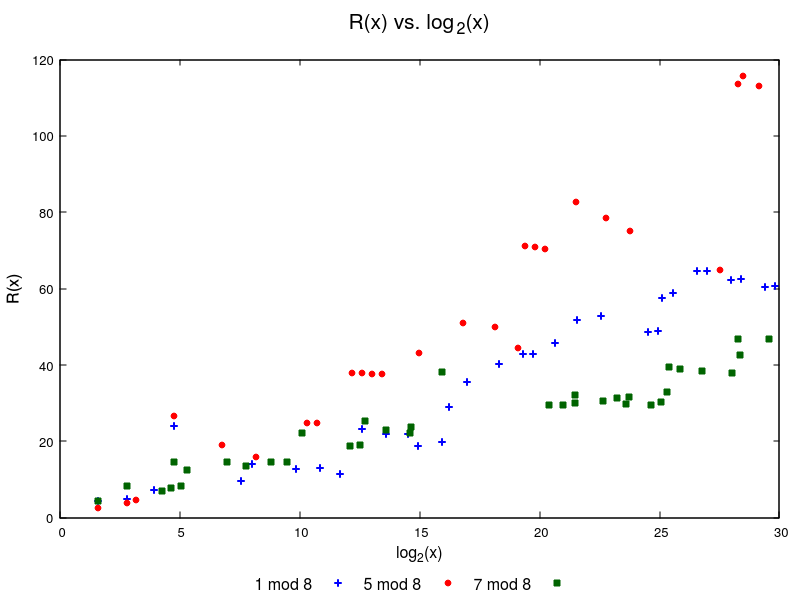
\includegraphics[scale=0.75]{ModAvoidanceAnalysisPics/R_vs_log.png}
    \caption{This graph visualizes how the $R$ values for subproblems 1, 5, and 7 compare to each other. The log of the record holding numbers, or number of bits needed, is the x-axis, and the hardness measure $R$ as defined in section~\ref{subsec:rewritemeasuredefs} is the y-axis.}
    \label{fig:rvslog}
\end{figure}
However, it is clear that all three cases don't have the same slope of increase. Subproblem 7 has the most gradual growth of all three cases, followed by subproblem 1 and subproblem 5, which has not only the most growth, but the highest standard deviation of all three cases. These can be explained by the following observations:
\begin{itemize}
    \item Record sequences for subproblem 7 eliminate the growth of the $6 \rightarrow 7 \rightarrow 6$ cycle, meaning the numbers tend to get smaller and need less bits to encode as a rewrite string.
    \item Record sequences for subproblem 5 eliminate the decay of the 0 self-cycle, meaning numbers tend to grow more often than not, so the numbers here are larger.
    \item Record sequences for subproblem 1 is in between the other two cases, since both the 0 self-cycle of decay and the $6 \rightarrow 7 \rightarrow 6$ of growth can occur.
\end{itemize}
